\chapter{Окружность}

\section{Форма и положение окружности}

\paragraph{}\label{1938/103}
\so{Предварительное замечание}.
Очевидно, что через одну точку ($A$, рис.~\ref{1938/ris-113}) можно провести сколько угодно окружностей:
центры их можно брать произвольно.
Через две точки ($A$ и $B$, рис.~\ref{1938/ris-114}) тоже можно провести сколько угодно окружностей, но центры их нельзя брать произвольно, так как точки, одинаково удалённые от двух точек $A$ и $B$, должны лежать на срединном перпендикуляре к отрезку $AB$ (§~\ref{1938/58}). 

\begin{figure}[!ht]
\begin{minipage}{.48\textwidth}
\centering
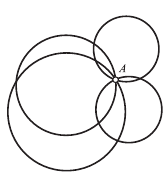
\includegraphics{mppics/ris-113}
\end{minipage}
\hfill
\begin{minipage}{.48\textwidth}
\centering
\includegraphics{mppics/ris-114}
\end{minipage}

\medskip

\begin{minipage}{.48\textwidth}
\centering
\caption{}\label{1938/ris-113}
\end{minipage}
\hfill
\begin{minipage}{.48\textwidth}
\centering
\caption{}\label{1938/ris-114}
\end{minipage}
\vskip-4mm
\end{figure}

Посмотрим, можно ли провести окружность через три точки.

\paragraph{}\label{1938/104}
\so{Теорема}.
\textbf{\emph{Через три точки, не лежащие на одной прямой, можно провести окружность и притом только одну.}}

Через три точки $A$, $B$ и $C$ (рис.~\ref{1938/ris-115}), только тогда можно провести окружность, если существует такая четвёртая точка $O$, которая одинаково удалена от точек $A$, $B$ и $C$.

\begin{wrapfigure}{o}{45mm}
\centering
\includegraphics{mppics/ris-115}
\caption{}\label{1938/ris-115}
\end{wrapfigure}

Докажем, что если $A$, $B$ и $C$ не лежат на одной прямой 
(другими словами, если точки $A$, $B$ и $C$ являются вершинами треугольника),
то такая точка $O$ существует и притом только одна.
Для этого примем во внимание, что всякая точка, одинаково удалённая от точек $A$ и $B$, должна лежать на срединном перпендикуляре $MN$, проведённом к стороне $AB$ (§~\ref{1938/58}); 
точно так же всякая точка, одинаково удалённая от точек $B$ и $C$, должна лежать на срединном перпендикуляре $PQ$, проведённом к стороне $BC$.
Значит, если существует точка, одинаково удалённая от трёх точек $A$, $B$ и $C$, то она должна лежать одновременно и на $MN$, и на $PQ$, что возможно только тогда, когда она совпадает с точкой пересечения этих двух прямых.
Прямые $MN$ и $PQ$ всегда пересекаются, так как они перпендикулярны к пересекающимся прямым $AB$ и $BC$ (§~\ref{1938/78}).
Точка $O$ их пересечения и будет точкой, одинаково удалённой от $A$, от $B$ и от $C$;
значит, если примем эту точку за центр, а за радиус возьмём отрезок $OA$ (или $OB$, или $OC$), то окружность пройдёт через точки $A$, $B$ и $C$.
Так как прямые $MN$ и $PQ$ могут пересечься только в одной точке, то центр такой окружности может быть только один, и длина её радиуса может быть только одна;
значит, искомая окружность — единственная.

{\small

\smallskip
\so{Замечание}.
Если бы три точки $A$, $B$ и $C$ (рис.~\ref{1938/ris-115}) лежали на одной прямой, то перпендикуляры $MN$ и $PQ$, были бы параллельны и, значит, не могли бы пересечься.
Следовательно, через три точки, лежащие на одной прямой, нельзя провести окружности.

}

\smallskip
\so{Следствие}.
Точка $O$ (рис.~\ref{1938/ris-115}), находясь на одинаковом расстоянии от $A$ и от $C$, должна также лежать на срединном перпендикуляре $RS$, проведённом к стороне $AC$. 
Таким образом:
\emph{три срединных перпендикуляра к сторонам треугольника пересекаются в одной точке.}

\paragraph{}\label{1938/105}
\mbox{\so{Теорема}.}
\textbf{\emph{Диаметр}} ($AB$, рис.~\ref{1938/ris-116}), \textbf{\emph{перпендикулярный к хорде}} ($CD$), \textbf{\emph{делит эту хорду и обе стягиваемые ею дуги пополам.}}
Перегнём чертёж по диаметру $AB$ так, чтобы его левая часть упала на правую.
Тогда левая полуокружность совместится с правой полуокружностью, и перпендикуляр $KC$ пойдёт по $KD$.
Из этого следует, что точка $C$, представляющая собой пересечение полуокружности с $KC$, совпадёт с $D$;
поэтому $CK=KD$,
${\smallsmile} BC={\smallsmile} BD$ и
${\smallsmile} AC={\smallsmile} AD$.

\paragraph{}\label{1938/106}
\mbox{\so{Обратные теоремы}.}

1.
\textbf{\emph{Диаметр}} ($AB$), \textbf{\emph{проведённый через середину хорды}} ($CD$)\textbf{\emph{, не проходящей через центр, перпендикулярен к этой хорде и делит дугу, стягиваемую ею, пополам}} (рис.~\ref{1938/ris-116}).

\begin{wrapfigure}{r}{33mm}
\centering
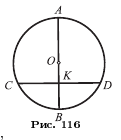
\includegraphics{mppics/ris-116}
\caption{}\label{1938/ris-116}
\end{wrapfigure}

2.
\textbf{\emph{Диаметр}} ($AB$), \textbf{\emph{проведённый через середину дуги}} ($CBD$), \textbf{\emph{перпендикулярен к хорде, стягивающей эту дугу, и делит её пополам.}}

Оба эти предложения легко доказываются от противного.


\paragraph{}\label{1938/107}
\mbox{\so{Теорема}.}
\textbf{\emph{Дуги}} ($AC$ и $BD$, рис.~\ref{1938/ris-117}), \textbf{\emph{заключённые между параллельными хордами}} ($AB$ и $CD$), \textbf{\emph{равны.}}

Перегнём чертёж по диаметру $EF\z\perp AB$.
Тогда на основании предыдущей теоремы можно утверждать, что точка $A$ совпадёт с $B$, точка $C$ совпадёт с $D$ и, следовательно, дуга $AC$ совместится с дугой $BD$, то есть эти дуги равны.


\begin{figure}[h]
\begin{minipage}{.32\textwidth}
\centering
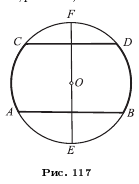
\includegraphics{mppics/ris-117}
\end{minipage}\hfill
\begin{minipage}{.32\textwidth}
\centering
\includegraphics{mppics/ris-118}
\end{minipage}\hfill
\begin{minipage}{.32\textwidth}
\centering
\includegraphics{mppics/ris-119}
\end{minipage}

\medskip

\begin{minipage}{.32\textwidth}
\centering
\caption{}\label{1938/ris-117}
\end{minipage}\hfill
\begin{minipage}{.32\textwidth}
\centering
\caption{}\label{1938/ris-118}
\end{minipage}\hfill
\begin{minipage}{.32\textwidth}
\centering
\caption{}\label{1938/ris-119}
\end{minipage}
\vskip-4mm
\end{figure} 

\paragraph{}\label{1938/108}
\mbox{\so{Задачи}.}
1) \emph{Разделить данную дугу \emph{($AB$, рис.~\ref{1938/ris-118})} пополам.}

Соединив концы дуги хордой $AB$, опускаем на неё перпендикуляр из центра и продолжаем его до пересечения с дугой.
По доказанному в предыдущей теореме, дуга $AB$ разделится этим перпендикуляром пополам.

Если же центр не известен, тогда к хорде $AB$ следует провести срединный перпендикуляр. 

2) \emph{Найти центр данной окружности} (рис.~\ref{1938/ris-119}).

Взяв на данной окружности какие-нибудь три точки $A$, $B$ и $C$, проводят через них две хорды, например $AB$ и $CD$, и проводят к ним срединные перпендикуляры $MN$ и $PQ$. 

Искомый центр, будучи одинаково удалён от $A$, $B$ и $C$, должен лежать и на $MN$ и на $PQ$, следовательно, он находится в их пересечении, то есть в точке $O$.

